%% $Id: zwpagelayout.tex 454 2013-01-13 18:30:27Z zw $
\input utf8-t1 % encTeX required
\documentclass[11pt]{article}
\usepackage{zwgetfdate}
\usepackage[footskip=30pt,topmargin=2cm,leftmargin=15mm,rightmargin=55mm,botmargin,nopdfinfo]{zwpagelayout}
\usepackage[T1]{fontenc}
\usepackage{lmodern,array,dcolumn,verbatim,graphicx}
\usepackage[figuresright]{rotating}
\usepackage[protrusion=false,expansion=true,stretch=8,shrink=24,step=4]{microtype}
\makeatletter
\renewcommand*\l@section{\@dottedtocline{1}{\z@}{1.5em}}
\makeatother
\extrarowheight 2pt
\mubytein 0 % important due to bug in url.sty
\usepackage[pdftitle=Page\ Layout\ with\ Crop\ Marks, pdfauthor=Zdenek\ Wagner,
            pdfkeywords={page layout,\ crop marks},
            bookmarks,bookmarksopen,bookmarksopenlevel=2]{hyperref}
\mubytein 1 \mubyteout 1 \mubytelog 1

\marginparwidth\UserRightMargin
\advance\marginparwidth -1cm
\advance\marginparwidth-\marginparsep

\def\mg#1{\ifvmode\leavevmode\fi\marginpar{\texttt{#1}}\ignorespaces}
\def\cmg#1{\mg{\char`\\#1}}
\def\omg#1{\ifvmode\leavevmode\fi\marginpar{\raggedright\hspace{0pt}\opt{#1}}\ignorespaces}
\def\opt#1{\texorpdfstring{\textmd{\textsc{#1}}}{#1}}
\let\pkg\textsc
\DeclareRobustCommand\cmd[1]{\texttt{\char`\\#1}}
\def\ie.{i.\,e.\@}
\def\eg.{e.\,g.\@}
\def\true{\bool{true}}
\def\false{\bool{false}}
\def\bool#1{\texorpdfstring{\textit{#1}}{#1}}
\def\is{\unskip\nobreak\space =\penalty200 \space\ignorespaces}

\DeclareRobustCommand\XeTeX{X\kern-.125em\lower.5ex\hbox{\csname
              reflectbox\endcsname{E}}\kern-.1667em\TeX}
\DeclareRobustCommand\XeLaTeX{X\kern-.125em\lower.5ex\hbox{\csname
              reflectbox\endcsname{E}}\LaTeX}

\makeatletter
\newcommand*\papdims[2][.]{\bgroup
    \def\zw@papdim##1,##2\zw@{\sepunit{##1}#1\sepunit{##2}}%
    \setkeys{zwpl}{#2}%
    \expandafter\zw@papdim\zwpl@papersize\zw@\egroup}

\newcommand*\sepunit[2][\,]{\def\zw@a{}\def\zw@x{#1}\def\zw@y{}\def\zw@z{}\zw@sepunit#2\zw@}
\def\zw@sepunit#1{\ifx#1\zw@
      \let\next\zw@sep@finished
    \else
      \edef\zw@a{\zw@a\zw@y}\edef\zw@y{\zw@z}\edef\zw@z{#1}\let\next\zw@sepunit
    \fi \next}
\def\zw@sep@finished{\zw@a\zw@x\mbox{\zw@y\zw@z}}
\makeatother

\def\krat{\,\ensuremath{\times}\,}

\newcolumntype{x}{D{.}{\krat}{-1}}
\def\xx#{\multicolumn{1}{c|}}

\let\zwcomma\,
\def\,{\texorpdfstring{\zwcomma}{}}

\clubpenalty10000
\widowpenalty10000

\begin{document}
\hyphenation{post-script ghost-script allow-with-height-switching Output-Condition Output-Condition-Identifier}

\title{Page Layout with Crop Marks}
\author{Zdeněk Wagner\\\url{http://icebearsoft.euweb.cz}}
\date{Package date: \DateOfPackage{zwpagelayout}}
\maketitle

\begin{abstract}\noindent
This package was developed as a typographers toolbox offering the most important features for
everyday work. First it allows setting the paper size as well as the page layout. The next
important feature is the ability of printing crop marks both with \TeX~+~dvips or (x)dvipdfm(x) and with pdf\TeX.
Finally it is possible to reflect pages both horizontally and vertically, select black overprint
and set various PDF/X features.
\end{abstract}

\tableofcontents

\section{Introduction}
Users will probably ask: ``Why another page layout package? Is not \pkg{geometry} all what we
need?'' The answer to this question is not easy. The \pkg{geometry} package provides a lot of
features, maybe even too many features. However, some features are missing. Packages for crop marks
can also be found but correct positioning of the crop marks requires cooperation with the
page layout package. It is therefore natural to integrate both these functions into a single
package.

The package is useful also for preparation of book covers. It places the marks showing the position
of a spine and optionally flaps. If you want to see whether the spine and the front and back cover
contents are properly aligned, you can display the frames. Moreover, it is often necessary to
create a proof of the cover while the book is not yet finished and the thickness of the spine is
not known and can be only approximated. You can thus leave the paper width empty and the package
will calculate it from the page width, the flap width and the spine thickness. Whenever the final
value of the spine thickness is known, you change it in the list of options and the whole layout
will adapt automatically.

The files usually fail to meet PDF/X conformance due to silly reasons. It is always mandatory to
set the title, creation date and modification date in any PDF file. It can be done by the
\pkg{hyperref} package. However, \pkg{hyperref} is a complex package that may cause clashes with
other packages. We do not want to kill ants by cannon balls, therefore we do simple things by simple
means. Options for partial PDF/X conformance were added but may be switched off if a user wishes to
use \pkg{hyperref}.

The package is a result of a long-term development inspired by author's everyday needs. It is a
collection of macros that were manually copied from document to document, later placed into private
packages and finally it matured into a package prepared for general use.

Being a result of development it may happen that you may be in the same situation in which I was
myself. The book was finished and the last task was to add the crop marks. Removing layout
definition from a document and replacing it with a different package may cause errors and one more
proof-reading is time consuming and expensive. This package therefore allows the page layout logic
to be switched off and just add the crop marks provided the paper dimensions are correctly
supplied. The details will be explained later when describing the package options.

\section{Package dependence}
As written in the introduction, the goal was to implement as much within this single package in
order to reduce the risk of clashes. Yet a few packages may be loaded. The package needs to know
what engine is being used. For this purpose the \pkg{ifxetex} and \pkg{ifpdf} packages are used. If
any of these packages is not found, it is assumed that the corresponding engine is not available.
No error is reported. The color support requires the \pkg{color} package. It is loaded only if the
color support is requested. The algorithm for deciding when the package is needed will be described
in detail in section~\ref{color}.

Option setting is implemented via the \pkg{kvoptions} package which in turn loads the \pkg{keyval}
package. These packages should be available in any nowaday's \TeX\ distribution.

\section{Usage}
The package is loaded simply by:

\vb
\verb;\usepackage[;$\langle$options$\rangle$\verb;]{zwpagelayout};

\vb\noindent
Remember that the options cannot be given later, all of them must be present either here or as
options to the \cmd{documentclass} command. The package will set some dimensions based upon
\cmd{normalsize}. The package that modifies font sizes must therefore be loaded before
\pkg{zwpagelayout}.

\section{Option values}

Some options accept a value. If the option is not specified, it may have a \textbf{default} value. For ease of use an
option may be given without a value. It will then have a \textbf{standard} value. The default and standard
values will be given in the option description.

The option value may sometimes contain spaces and commas. However, commas are used to separate
options, and during parsing the spaces are ignored. The spaces must therefore be preceded by a
backslash and an option value containing commas must be enclosed in braces, for example:

\vb
\begin{verbatim}
\usepackage[a4,subject=Some\ subject,
            keywords={keyword\ 1,\ keyword\ 2}]{zwpagelayout}
\end{verbatim}

\section{Driver selection}\label{driver.selection}
The driver is usually selected automatically. The package makes use of the \pkg{ifxetex} and
\pkg{ifpdf} packages to detect either \XeTeX\ or pdftex. If none of them is detected, dvips is
assumed.

\omg{driver}
It may sometimes be necessary to set the driver manually by giving the \opt{driver} option. This
option recognizes drivers \texttt{unknown}, \texttt{pdftex}, \texttt{xetex}, and \texttt{dvips}. In
addition \texttt{other} is an alias to \texttt{unknown}, \texttt{dvipdfm} and \texttt{xdvipdfmx}
are aliases to \texttt{xetex}.

The package shows the driver in the log file. If the driver is set to \texttt{unknown}, all driver
specific features will be disabled.

\section{Paper size and orientation}
The first task of the package is to define paper size and orientation. Remember that the package is
intended for use in real life where we cannot be limitted to standard papers sizes. However, the
standard paper sizes are used quite often and we must be able to use them too. The options were
tested with pdf\TeX, \pkg{dvips} as well as \pkg{(x)dvipdfm(x)}.

\subsection{Orientation}\label{orientation}
\omg{AllowWidthHeightSwitching}
The package usually accepts the dimentsions as they are, \ie. width and height of the page. The
orientation cannot be changed. If you wish to have the possibility to change the orientation, you
have to use this option. It is used automatically with all standard paper sizes (see
section~\ref{standard}). You will rarely specify it yourself.

\omg{Portrait}\omg{Landscape}
These options sets the paper orientation, \opt{Portrait} is the default. They can be used only if
\opt{AllowWidthHeightSwitching} was specified, otherwise they are ignored.

\subsection{Paper size}
The package option defines the trimmed paper size. If the crop marks are added, the real paper size
will be added. Dimensions \cmd{paperwidth} and \cmd{paperheight} will thus contain the values that
will subsequently be sent to the driver. If you for any reason wish to know the trimmed dimensions,
you can calculate them as follows:

\begin{center}
trimmed width = \cmd{paperwidth} -- 2\cmd{hoffset}

trimmed height = \cmd{paperheight} -- 2\cmd{voffset}
\end{center}

\subsubsection{Generic paper size}
\omg{papersize}
Option \opt{papersize} is used to define arbitrary paper size. You define it as a pair of two
dimensions, the width and the height. The numbers are separated by a comma, therefore the
specification must be enclosed within braces, \eg.

\begin{verbatim}
\usepackage[papersize={200mm,100mm}]{zwpagelayout}
\end{verbatim}

The above written command sets the paper width to 200\,mm and the paper height to 100\,mm, \ie. the
paper orientation will be landscape. Now consider the following:

\begin{verbatim}
\usepackage[papersize={200mm,100mm},
    AllowWidthHeightSwitching]{zwpagelayout}
\end{verbatim}

Since the width/height switching is allowed and the default orientation is portrait (option
\opt{Portrait} is the default), the width will be 100\,mm and the height will be 200\,mm.

You can achieve the same result as the first command by the lengthy code:

\begin{verbatim}
\usepackage[papersize={200mm,100mm},
    AllowWidthHeightSwitching,Landscape]{zwpagelayout}
\end{verbatim}

You see that the command may become confusing. You should better not use
\opt{AllowWidthHeightSwitching} together with \opt{papersize}.

If the \opt{papersize} option is not used, it defaults to the A4 size, \ie. to paper dimensions \papdims[\krat]{a4}.

If the book cover is being typeset, we want to calculate at least the width. The detailed
explanation will be given in section~\ref{missing}. Here we put just as an example:

\begin{verbatim}
\usepackage[papersize={,200mm},spine=15mm,textwidth=14cm,
            margins]{zwpagelayout}
\end{verbatim}

It is even possible to calculate both dimensions using \eg.

\begin{verbatim}
\usepackage[papersize,spine=15mm,textwidth=14cm,textheight=20cm,
            margins]{zwpagelayout}
\end{verbatim}

\subsubsection{Standard paper sizes}\label{standard}
\omg{a0\,\ldots\,c10}\omg{executive}\omg{legal}\omg{letter}
Options \opt{a0}\ldots\opt{a10}, \opt{b0}\ldots\opt{b10}, \opt{c0}\ldots\opt{c10} are used to
select paper size according to the A, B or C series where the dimensions are rounded to integers in
milimeters. For instance, the A6 size is \papdims[\krat]{a6}. The package also supports paper sizes
\opt{executive} (\papdims[\krat]{executive}), \opt{legal} (\papdims[\krat]{legal}), and
\opt{letter} (\papdims[\krat]{letter}). If one of these options is used,
\opt{AllowWidthHeightSwitching} and \opt{Portrait} are assumed. The page orientation may be
switched by option \opt{Landscape} (see section~\ref{orientation}).

\subsection{Page bounding boxes}\label{Bboxes}
The drivers usually set MediaBox to the physical size of the page. If cropmarks are requested (see
section~\ref{cropmarks}), the package sets also BleedBox and TrimBox, ArtBox is explicitely
forbidden by PDF/X. CropBox is
intentionally unset since it causes cropped display in Adobe Reader. Since page size setting is
delayed, MediaBox contains the whole page including the area for the cropmarks. MediaBox is
calculated by the driver, the other boxes are calculated by \TeX. Their dimensions are therefore
not exact because \TeX\ does not use floating point arithmetic. The difference is negligible.

\omg{noBboxes}
Option \opt{noBboxes} disables setting the above mentioned boxes. Currently there is a known bug
causing fatal error in Adobe Distiller if these boxes are set.

\cmg{noBboxes}
Macro \cmd{noBboxes} performs exactly the same action as the \opt{noBboxes} option. The only
advantage is that it can be used later in the preamble of the document. It cannot be used after
\verb.\begin{document}. because the boxes are already set at that time.

\section{Page layout options}
These options define the layout of the odd page. The layout of the even page is assumed to be a mirror image.
The values of \cmd{oddsidemargin} and \cmd{evensidemargin} are calculated from the values of the options.

\subsection{Margins}
This set of options us used to define margin sizes.
Remember that all margins are measured from the top left corner of the paper, not from 1in border which is
the \textsc{dvi} origin!

\subsubsection{Option \opt{margins}, standard 0\,mm}
\omg{margins}
This option sets all margins (top, left, right, bottom) to the specified size. You will not be able to change
some of the margin to another size. If you need different size for any margin, you have to set all of them
separately and not use this option. Notice that almost everything may be calculated automatically, thus it is
not necessary to specify all values.

\subsubsection{Option \opt{topmargin}, default 1\,in}
\omg{topmargin}
This option sets the value of \cmd{topmargin}.

\subsubsection{Option \opt{botmargin}, standard \opt{topmargin}}
\omg{botmargin}
This option specifies the size of the margin below the running footer.

\subsubsection{Option \opt{leftmargin}, default --1\,in}
\omg{leftmargin}
This option sets the value of the margin at the left side of an odd page (and the margin at the right side of
an even page). Negative value means that the value was not given.

\subsubsection{Option \opt{rightmargin}, default --1\,in}
\omg{rightmargin}
This is the size of the right side of an odd page. Similarly the negative value means that the option was not
specified.

\subsection{Text dimensions}
The following options are used to specify the height and width of the text.

\subsubsection{Option \opt{textwidth}, default --1\,in}
\omg{textwidth}
This option specifies the width of the text without marginal notes. Its meaning is different for
book covers. The option specifies the width of the cover without the extra spine (\opt{xspine}),
flap (\opt{flap}) and trimming (\opt{xtrim} or \opt{trim}).

\subsubsection{Option \opt{textheight}, default --1\,in}
\omg{textheight}
This option specifies the total height of the text including the header and footer.

\subsubsection{Option \opt{headheight}, default 0\,mm}
\omg{headheight}
This option specifies the height of the running head.

\subsubsection{Option \opt{headsep}, default 0\,mm}
\omg{headsep}
This is the value of \cmd{headsep}.

\subsubsection{Option \opt{footskip}, default 0\,mm}
\omg{footskip}
This option specifies the value of \cmd{footskip}.

\subsubsection{Option \opt{topskip}\texorpdfstring{, default \cmd{topskip}}{}}
\omg{topskip}
This option enables changing the value of \cmd{topskip}. It is rarely needed. However, the value of
\cmd{topskip} is usually less than \cmd{baselineskip} which may cause problems in some page layout schemes.
Since we have already written that font sizes must be defined before \pkg{zwpagelayout} is loaded, you can
safely specify \verb;topskip=\baselineskip;.

\subsubsection{Option \opt{strictheight}, default \false, standard \true}
\omg{strictheight}
The value of the \LaTeX\ dimension \cmd{textheight} is calculated from the values of the options and later
adjusted so that together with \cmd{topskip} it represents an integer number of lines. This may not be
desirable in some cases. This option instructs the package not to perform any adjustment and accept the
calculated value.

\subsubsection{Option \opt{adjustfootskip}, default \true, standard \true}
\omg{adjustfootskip}
If option \opt{strictheight} is not given, the calculated value of \cmd{textheight} is decreased to the nearest
integer multiple of \cmd{baselineskip}. The difference is then added to \cmd{footskip} in order to preserve to
total height. If \opt{adjustfootskip} is set to \false, the difference is added to \cmd{headsep} instead.

\begin{figure}[bt]
\noindent
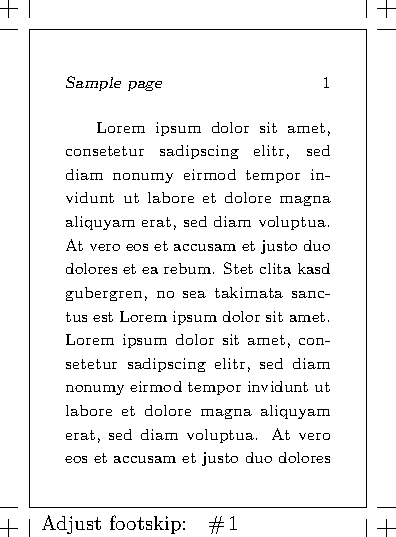
\includegraphics{adjustfoot}\hfill
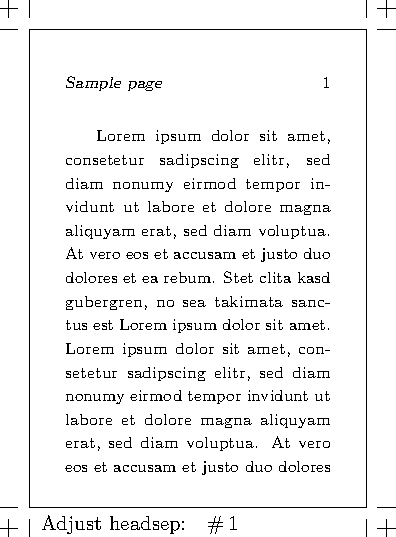
\includegraphics{adjusthead}

\vb
\caption{Compensation of \cmd{textheight} by changing \cmd{footskip} (on the left) and
\cmd{headsep} (on the right)}\label{adj}
\end{figure}

The difference betweem these two options is shown in figure~\ref{adj}. Adjustment of \cmd{footskip}
was achieved by:

\vb
\begin{verbatim}
\usepackage[c8,margins=6mm,headheight=4mm,headsep=4mm,
   croplength=3mm,cropgap=2mm,
   cropmarks,cropframe,croptitle=Adjust\ footskip]{zwpagelayout}
\end{verbatim}

\vb \noindent
The sample on te right side of the figure was created by:

\vb
\begin{verbatim}
\usepackage[c8,margins=6mm,headheight=4mm,headsep=4mm,adjustheadsep,
   croplength=3mm,cropgap=2mm,
   cropmarks,cropframe,croptitle=Adjust\ headsep]{zwpagelayout}
\end{verbatim}

\subsubsection{Option \opt{adjustheadsep}, default \true, standard \true}
\omg{adjustheadsep}
This is a complementary option to \opt{adjustfootskip}.

\section{Calculation of missing dimensions}\label{missing}
The package can either calculate paper size from the page layout dimensions or calculate missing
page layout dimensions if the paper size and some dimensions are known. It operates separately for
the height and width. You can \eg. define the paper height and calculate the text height from it
and the margins but specify all width layout dimensions and calculate the paper width.

When designing simple pages it is better to define the paper size and calculate some page layout
dimensions. However, for bok covers it is recommended to calculate at least the paper width from
the layout dimensions of the front cover, the spine and the flap width.

\subsection{Calculation of the paper size}
Remember that paper size can be calculated only if all page layout dimensions for the corresponding
orientation (height, width) are specified. There is no diagnostics for warning you if some
important options are missing, the resukt will just be wrong or the package may even report an
error. All dimensions are considered \emph{without} the area for the crop marks.

\subsubsection{Paper height}
Calculation of the paper height is very simple. The formula is:

\vb
\cmd{paperheight} = \opt{topmargin} + \opt{textheight} + \opt{botmargin} + 2 \opt{ytrim}

\vb \noindent
Remember that \opt{textheight} includes also \cmd{headheight}, \cmd{headsep}, and \cmd{footskip}.
It is not necessary to specify \opt{ytrim}, the package checks the existence of this option and
removes it from the formula if not given.

\subsubsection{Paper width}
Algorithm for calculating the paper width differs for simple pages and book covers. In the simple
case the paper width is calculated as follows:

\vb
\cmd{paperwidth} = \opt{leftmargin} + \opt{textwidth} + \opt{rightmargin}

\vb \noindent
The value of \cmd{textwidth} will be equal to \opt{textwidth}. The same value will be stored in
macro \cmd{UserWidth}, see section~\ref{crop.macros}.

If the book cover is designed, the \opt{textwidth} option refers to the width of the text at the
front cover but \opt{leftmargin} and \opt{rightmargin} are used to set \cmd{oddsidemargin} and
\cmd{evensidemargin}. It is therefore better to set these options to zero, or alternatively to the
same value as \opt{flap} or \opt{xtrim} if the corresponding area will be left empty. The value of
\cmd{textwidth} will then be calculated from the final paper width by:

\vb
\cmd{textwidth} = \cmd{paperwidth} -- \opt{leftmargin} -- \opt{rightmargin}

\vb
If the \opt{flap} option is used without the \opt{spine} option in order to emulate the front cover
and spine with an empty back cover, the paper width is calculated as:

\vb
\cmd{paperwidth} = \opt{leftmargin} + \opt{flap} + \opt{textwidth} + \opt{xtrim} +
\opt{rightmargin}

\vb \noindent
The value of \opt{xtrim} may be omitted. The value of \opt{xspine} will be silently ignored. It is
not allowed to have just the spine, the front cover and the flap while leaqving the back cover
empty.

The case of a book cover with the spine given is a bit more complicated:

\vb
\textit{width} = \opt{xspine} + \opt{textwidth} + \opt{flap} + \opt{xtrim}

\cmd{paperwidth} = \opt{leftmargin} + \opt{spine} + 2 \textit{width} + \opt{rightmargin}

\vb \noindent
Options \opt{xspine}, \opt{flap}, and \opt{xtrim} need not be specified if these elements are not
needed.

\subsection{Calculation of page layout dimensions}\label{calc.pg.layout}
Algorithm for calculating the page layout dimensions is intended for simple pages, not for book
covers. Options \opt{xtrim}, \opt{ytrim}, \opt{spine}, \opt{xspine}, and \opt{flap} are silently
ignored but will be taken into account when producing the crop marks. You can still make use of
this algorithm if you understand what you are doing and if you wish to do extra calculations
yourself.

The dimensions may be overdetermined. In such a case the algorithm disregards one of the dimensions
and calculates it.

\subsubsection{Vertical dimensions}\label{vert.dim}
The algorithm first looks whether \opt{textheight} was given. If not it is assumed that the user
wishes to have it calculated from the paper height and the margins. If the \opt{botmargin} option was
not set, it will be set to the same valu as \opt{topmargin}.

In the second step the package looks whether \opt{botmargin} is defined, either by the user or from
the previous step. If so, the text height is calculated, otherwise the bottom margin is calculated
from the top margin and the text height. As a matter of fact, the bottom margin is never used by
\TeX.

Finally the value of \cmd{textwidth} is reduced by \cmd{headheight}, \cmd{headsep}, and
\cmd{footskip}. If \opt{strictheight} is \cmd{false}, the values are later adjusted according to
options \opt{adjustfootskip} and \opt{adjustheadsep} so that \cmd{textheight} -- \cmd{topskip} is
an integer multiple of \cmd{baselineskip}.

\subsubsection{Horizontal dimensions}
The sum of the horizontal dimensions must be equal to the paper width according to the relation:

\vb
\opt{leftmargin} + \opt{textwidth} + \opt{rightmargin} = \cmd{paperwidth}

\vb \noindent
If all three dimensions are specified, \opt{textwidth} is disregarded and calculated from the other
dimensions. If any two dimensions are given, the missing one is calculated from the above formula.
If only one dimension is given, it is assumed that both margins have the same size and the above
formula is applied. It is even possible to omit all dimensions. In such a case the margins are
assumed to have the same size as \opt{topmargin} and the text width can thus be calculated.

\section{Page reflection}\label{reflection}
\omg{Reflect\-Horizontally}
\omg{ReflectVertically}
We sometimes need to print the whole document as a mirror image. Although there are external tools
that can provide such a job taking PDF or PS as input, it is useful to do everything in a single
step. The package provides options \opt{ReflectHorizontally} for horizontal reflection and
\opt{ReflectVertically} for vertical reflection, respectively. If you specify both, some drivers
may interpret both of them and print rotated 180$^{\circ}$, some interpret only one of them.

The PostScript to PDF converters optionally rotate pages according to the text direction. They may
be confused by reflected text and add undesired rotation. If the horizontally reflected text is
roteted 180$^{\circ}$, it looks as if it were reflected vertically instead.

Remember that these options are intended for printing only.
The hypertext links made by the \pkg{hyperref} package will be wrong. If you wish to rotate parts
of texts and preserve hyperlinks, use \pkg{rotating} instead.

A word of warning has to be said. In \texttt{pdftex} reflection is implemented by redefininng
\cmd{shipout}. We add PDF literal code to the beginning of each page. For \texttt{dvips} we add
code to the \texttt{bop-hook}. If you need your own code in the \texttt{bop-hook}, you have to
store the old definition and execute it. For \texttt{xetex} we add code to \texttt{bop} and
\texttt{eop}. It seems that only one \texttt{bop} and one \texttt{eop} can be used. That is why the
page is reflected vertically if both options are used. As a result you are not allowed to use your
own \texttt{bop} and \texttt{eop} code together with these options.

\section{Crop marks}\label{cropmarks}
The crop marks must appear outside the print area. The package assumes that \cmd{paperheight} and
\cmd{paperwidth} contain the page size after trimming. These dimensions will then be increased and the page
will be shifted by setting \cmd{hoffset} and \cmd{voffset}. If you wish to print the crop marks using
\opt{zwpagelayout}, you must not change values of \cmd{hoffset} and \cmd{voffset}.

The values of \cmd{hoffset} and \cmd{voffset} will be set to the sum of \opt{croplength} and \opt{cropgap}, see the following
text.

\subsection{Basic crop marks options}
Options described in this section define basic behaviour of the crop marks. The options can be used
in all crop mark styles.

\subsubsection{Option \opt{onlycropmarks}, default \false, standard \true}
\omg{onlycropmarks}
It may happen that a document is already finished and proof-read and just the crop marks have to be added.
By specifying option \opt{onlycropmarks} you instruct the package to ignore all page layout options and
interpret the crop marks options only. You just have to ensure that \cmd{paperheight} and \cmd{paperwidth} are
set to the dimensions of the trimmed page before the \pkg{zwpagelayout} package is loaded and \cmd{hoffset} and
\cmd{voffset} are left at their default values.

\subsubsection{Option \opt{cropmarks}, default \false, standard \true}
\omg{cropmarks}
This option asks for creation of the crop marks.

\subsubsection{Option \opt{nocropmarks}, default \true, standard \true}
\omg{nocropmarks}
This is a complementary option to \opt{cropmarks}.

\subsubsection{Option \opt{croplength}, default 5\,mm}
\omg{croplength}
This option specifies the length of the crop mark.

\subsubsection{Option \opt{cropgap}, default 5\,mm}
\omg{cropgap}
This is the space that must be left blank between the crop marks and the trimmed page. This area is
also known as bleed.

\subsubsection{Option \opt{cropframe}, default \false, standard \true}\label{cropframe}
\omg{cropframe}
When designing a book cover we often wish to verify whether all elements are properly aligned.
Option \opt{cropframe} can be used to print the frames. It is active only if \opt{cropmarks} was
specified.

\subsubsection{Option \opt{nocropframe}, default \true, standard \true}
\omg{nocropframe}
This is a complementary option to \opt{cropframe}.

\subsubsection{Option \opt{cropstyle}}\label{cropstyle}
\omg{cropstyle}
This option selects the style of the crop marks. Two styles are defined, \textit{default} and
\textit{leaflet}.

\subsubsection{Option \opt{croptitle}}
\omg{croptitle}
This option defines the text that should be printed on each page. It may \eg. be the title of the
document. Remember that all spaces are gobbled when parsing the options. The spaces must therefore
be specified as \verb*;\ ; or the text must be enclosed in curly braces.

\subsubsection{Option \opt{cropseparator}}
\omg{cropseparator}
This is the separator between the title and the page number. Its default value is \verb;:\quad;.

\subsubsection{Option \opt{pagenumberfirst}, default \false, standard \true}
\omg{pagenumberfirst}
Each page contains the title followed by the separator and the page number. If you set this
option to \true, the order will be reversed.

\subsubsection{Option \opt{pagenumberlast}, default \true, standard \true}
\omg{pagenumberlast}
This is a complementary option to \opt{pagenumberfirst}.

\subsubsection{Option \opt{usepagenumbers}, default \true, standard \true}
\omg{usepagenumbers}
This option requests printing the page numbers.

\subsubsection{Option \opt{nopagenumbers}, default \false, standard \true}
\omg{nopagenumbers}
This is a complementary option to \opt{usepagenumbers}.

\iffalse
\subsubsection{Option \opt{cropfontsize}}
\omg{cropfontsize}
This option defines the font size command issued just before the title and page number are printed.
The default command is \verb;\fontsize{10}{10};.

\subsubsection{Option \opt{cropfont}}
\omg{cropfont}
This option contains the command to select a font for the title and the page number. The default
command is \cmd{normalfont}.
\fi

\subsubsection{Option \opt{nobleedclip}, default \false, standard \true}
\omg{nobleedclip}
The pages are clipped to the bleed box so that graphics does not collide with the crop marks. Since
the package must work also with \pkg{dvips}, the PDF operators are not used and the crop marks area
outside the bleed box is just overpainted with white rectangles. The \pkg{color} package is thus
required and will be loaded automatically. If you set \opt{nobleedclip} to \true, the pages will
not be clipped. It may be useful if you know that nothing extends to the crop marks area and the
\pkg{color} package may clash with other packages required by your document.

\subsection{Options for the \textit{default} style}
These options can be used if \opt{cropstyle} is set to \textit{default} or omitted.

\subsubsection{Option \opt{spine}}
\omg{spine}
This option is used for designing book covers. It specifies the width of the book spine. You can
even request a zero width but negative values will have disastrous results.

\subsubsection{Option \opt{xspine}}
\omg{xspine}
This option defines the extra space adjacent to the spine so that the book can be safely opened.
This space should not be used for printing logos etc., because they will soon be damaged by
frequent use of the book. The option is ignored unless \opt{spine} is used.

\subsubsection{Option \opt{flap}}
\omg{flap}
This is another option for book covers. It specifies the width of the flap. If \opt{spine} is
given, the book cover is supposed to have flaps of equal sizes on both sides. Sometimes you do not
have flaps and the back cover remains empty, thus you do not like to prepare the design of it, you
just wish to design the spine and the front cover. This can be acheved by specifying \opt{flap} as
the spine thickness and omitting \opt{spine}.

\subsubsection{Options \opt{trim}, \opt{xtrim}, \opt{ytrim}}
\omg{trim}\omg{xtrim}\omg{ytrim}
The paper or canvas used for printing the book covers is folded to the inner side yet part of it
will be visible. Such part is specified by \opt{xtrim} in horizontal direction and \opt{ytrim} in
vertical direction. You can use \opt{trim} to set both of them to the same value.

\subsection{Options for the \textit{leaflet} style}\label{cropstyle.leaflet}
The following options can be used if \opt{cropstyle} is defined as \textit{leaflet}. As the value
says, the style is useful for leaflet production because in addtion to the crop marks additional
marks for folding. Not all options can be used with all fold types. It will be described in greater
detail in the following text.

The leaflets are usually printed on both sides and sometimes one of the leaves needs width
correction as will be explained later. The macros will apply the correction the one side on odd
pages and on the other side on even pages. This can only happen if the \opt{twoside} class option
is given or a class is used where two-side printing is the default. Usually the leaflet will
consist of two pages only but no check is made.

The \opt{cropframe} option (see~\ref{cropframe}) can also be used for previewing the leaflet
layout.

\subsubsection{Option \opt{leafcount}, default 4}
\omg{leafcount}
This option defines the number of leaves to be used in the Z-type. It is silently ignored with
other fold types. Internally other fold types overwrite it with the value they need in the macros.

\subsubsection{Option \opt{foldcorr}, default 0mm}
\omg{foldcorr}
As default all leaves have equal width. However, from technical or stylistic reasons the letmost or
righmost leaf requires a different width. This can be achieved by this option. The value specifies
an additional horizontal skip that is applied when printing the crop/fold marks and the optional
frames.

The width of the leaves is equal because it is achieved by \cmd{hfil}. If you specify
\verb.foldcorr=-2mm., the corrected leaf will be 2\,mm narower that the others. Since there is
\textit{1fil} in the width specification of the leaves, you can achieve nice tricks be specifying
\verb.foldcorr=5cm plus -1fil.. In such a case the \textit{1fil} in the corrected leaf will vanish
and its width will be 5\,cm.

Width corrections are not allowed in the \textit{Z} and \textit{4} types and the option value is
ignored. The details of the \opt{foldcorr} will be given in the next section.

\subsubsection{Option \opt{fold}, default 2}
\omg{fold}
This option selects a fold type used with the leaflet. Supported options are \textit{2},
\textit{3left}, \textit{3right}, \textit{4}, \textit{Z}. Their exact meaning is described below.

\begin{description}
\item[2] This option is used for singly folded leaflet. Usually the leaves will have different
widths. The width of the left leaf is modified by the \opt{foldcorr} option.
\item[3left] This option defines a leaflet with three leaves folded inside. For technical reasons
the leaf folded inside must be slightly narrower. Typically this is the leftmost leaf. The leaf can
be made narrower by applying \opt{foldcorr}.
\item[3right] This is essentially the same as the previous option with the only difference that the
\opt{foldcorr} correction is applied to the rightmost leaf.
\item[Z] This option is used for Z-folded leaflets. The number of leaves is defined by the
\opt{leafcount} option and with correction is not allowed.
\item[4] This type of leaflet looks as the Z-type but without a fold in the middle. It can be
viewed as a middle leaf of double width and the outer leaves are folded so that they touch each
other. The middle crop mark is therefore missing because there is no fold there but a line will be
drawn if the \opt{cropframe} option is requested.
\end{description}

As a final remark it is important to write that the width correction is applied as explained above
on the odd pages. The correction of the same size is applied to the opposite side of the leaflet on
even pages.

\section{Color support}\label{color}
The package offers basic color support, namely it prints the names of separations. The
color support is implemented via a few options. Color printing is performed using the \pkg{color}
package that is loaded automatically. The package does not use predefined color names.

The package recognizes the \pkg{color} package by existence of the \cmd{definecolor} macro. If this
macro is not defined, the \pkg{color} package will be added if:
\begin{itemize}
\item option \opt{color} is \true
\item option \opt{nobleedclip} is \false\ and \opt{cropmarks} is \true
\item option \opt{redefineblack} is \true
\item option \opt{redefinetocmyk} is \true
\item option \opt{overprint} is \true
\end{itemize}
If none of the above applies, the color support is not needed and the package will not be loaded.

If the \pkg{color} package is being loaded, no options are given to it. Especially the driver
selected by the \opt{driver} option (see section~\ref{driver.selection}) is not set. If you must
specify any option for the \pkg{color} package, you have to load it yourself before loading
\pkg{zwpagelayout}.

\subsection{Color support for cropmarks}
\omg{color}
Option \opt{color} asks for the color support. Without setting this option to \true\ all other
color options are silently ignored.

\omg{colormodel}
Option \opt{colormodel} defines the color model used. Its default value is \texttt{cmyk}. You will
rarely need to change it.

\omg{cropcolor}
Option \opt{cropcolor} specifies the color to be used for the crop marks. Remember that the crop
marks must be visible on all separations, thus it might not be sufficient to print them in black.
As default their color is mixed of 100\,\% of all components of the current color model. Since the
default model is \texttt{cmyk}, the default value of this option is \verb;{1,1,1,1};. Notice that the
syntax conforms to the requirements of the \pkg{color} package.

\omg{colors}\label{colors}
Option \opt{colors} assigns names to the color components of the current model. Specification of
each color must be enclosed in curly brackets. The color name is followed by a colon and comma
separated values conforming to the syntax of the \pkg{color} package. It will be clear from the
following examples.

Suppose that for some strange reason you prepare the document in the RGB space. Your specification
will then be:

\vb

\begin{verbatim}
\usepackage[cropmarks,color,colormodel=rgb,cropcolor={1,1,1},
    colors={{RED:1,0,0},{GREEN:0,1,0},{BLUE:0,0,1}},
    croptitle=RGB\ example]{zwpagelayout}
\end{verbatim}

\vb

Now we show a more realistic example. The document should be printed in custom colors. Since the
true specification of custom colors requires much work and is rarely worth the trouble, we make use
of the CMYK model. We will use cyan instead of Pantone 298 (blue), magenta instead of Pantone 213
(red), black will remain black and the yellow separation will be unused. The crop marks should not
produce anything on the yellow separation and we should provide proper color names. The
specification will therefore look as:

\vb

\begin{verbatim}
\usepackage[cropmarks,color,cropcolor={1,1,0,1},
    colors={{Pantone\ 298\ (blue):1,0,0,0},
            {Pantone\ 213\ (red):0,1,0,0},{Black:0,0,0,1}},
    croptitle=Example\ with\ custom\ colors]{zwpagelayout}
\end{verbatim}

\vb

Notice that the \opt{colormodel} option was not specified. Its default value was used. The
\opt{cropcolor} option left zero for the yellow separation.

If a color is light as e.\,g. the process yellow, it may be better to display its name in white on
a colored background. This is achieved by preceding the color name with an asterisk. This is now
the default behaviour for the yellow color. The default definition is:

\vb
\begin{verbatim}
colors={{CYAN:1,0,0,0},{MAGENTA:0,1,0,0},{*YELLOW:0,0,1,0},{BLACK:0,0,0,1}}
\end{verbatim}

\vb

\subsection{CMYK colors}\label{cmykcolors}
\mg{cmykblack}\mg{cmykread}\mg{cmykgreen}\mg{cmykblue}
The \pkg{color} package defines \textit{black} using the GRAY model and colors \textit{red},
\textit{green}, \textit{blue} by the RGB model. The GRAY model rarely causes any problem but the
RGB model is not acceptable for printing. The \opt{zwpagelayout} package therefore defines the
corresponding colors using the CMYK model. Different names are selected so that there is no clash
in case you really need these colors in RGB.

\subsection{Overprinting support, default \false, standard \true}\label{overprinting}
\omg{overprint}
The overprinting support must be requested by the \opt{overprint} option. If the option remains
\false, the overprinting commands will be defined but will do nothing. Remember that you can
overprint any color, not just black. You thus should not enable overprinting globally. The mode is
therefore set to \textit{knockout} within the package.

\cmg{OverprintXeTeXExtGState}
Overprint is implemented in all supported drivers. However, there is a minor problem with the
(x)dvipdfm(x) family of drivers. The definition of the graphic state must be present in the
resources of each page where overprinting is used. The (x)dvipdfm(x) drivers do not do it
automatically, it has to be done by the \cmd{OverprintXeTeXExtGState} macro. Since the cropmarks
switch overprint off, they require the definition of the graphic state and the macro is always
invoked from the running head. This requirement is thus a minor problem. The user usually does not
care whether overprint is enabled for preview and proof-reading. The final document will have
cropmarks and thus overprint will be enabled.

\cmg{SetOverprint}\cmg{SetKnockout}
These macros change the mode to \textit{overprint} or \textit{knockout}, respectively. They act as
declarative macros, similarly as \eg. \cmd{itshape}. You have to use them within a group. The
macros are intended to be used for changing the mode for a longer part of text. Due to the way how
environments are handled in \LaTeX, it is also possible to write:

\vb
\begin{verbatim}
\begin{SetOverprint}
Some long text to be overprinted...
\end{SetOverprint}
\end{verbatim}

\vb

\cmg{textoverprint}\cmg{textknockout}
If a short part of text should be printed in a different mode, one-argument macros
\cmd{textoverprint} and \cmd{textknockout} can be used. They act similarly as the \cmd{textit}
macro.

\omg{redefineblack}
Overprinting works only if both the background and forground colors are in the CMYK model. However,
the \textit{black} color, which is most often overprinted, is defined in the GRAY model as default.
This package defines the \texttt{cmykblack} color that may be used for this purpose. In addition if
\opt{redefineblack} is set to \true, the standard \textit{black} color will be redefined in CMYK.

\omg{redefinetocmyk}
Although \textit{red}, \textit{green}, \textit{blue} will rarely be used for overprinting (maybe
just as a background), option \opt{redefinetocmyk} requests redefinition of these colors to CMYK.
The \textit{black} color will be redefined as well.

\vb
\textbf{Important note:} the (x)dvipdfm(x) drivers may switch to the gray colour model after
\cmd{textcolor} even if redefinition of black or even all colours to CMYK was requested. If black
overprint does not work, insert explicit \verb;\color{cmykblack};. This trick is not needed with
pdf\TeX\ or dvips.

\vb

\mg{grblack}\mg{rgbred}\mg{rgbgreen}\mg{rgbblue}
If the colors are redefined to CMYK, the original definitions are not available. Although you
redefine them due to a printing process where the RGB colors are undesirable, you can sometimes
need them. For this purpose \textit{grblack}, \textit{rgbred}, \textit{rgbgreen}, \textit{rgbblue}
colors are always available.

\section{PDF information}\label{pdfinfo}
The package writes the basic information that is required by PDF/X even if PDF/X conformace is not
requested. The basic pieces of information are \texttt{CreationDate} and \texttt{ModDate}.
Implementation is driver dependent and some information is supplied by the driver itself. Thus
\texttt{pdftex} inserts both, (x)dvipdfm(x) (\XeTeX) adds \texttt{CreationDate} only, dvips adds
none. The missing information is supplied by this package based on \cmd{date} and \cmd{time}. The
next subsections will explain how other fields can be defined and how they can be disabled if
needed.

\subsection{PDF title}\label{pdftitle}
\omg{title}
The \opt{title} option is used to set the title field. The default is to take the contents of the
\opt{croptitle} option even if the cropmarks are switched off. If \opt{croptitle} is empty,
\cmd{jobname} is used. If you specify this option without a value, it has a special meaning of
suppressing creation of PDF information field. Since this is not mnemonic, there is a
\opt{nopdfinfo} option with the same effect, see subsection~\ref{nopdfinfo}.

\subsection{PDF author}
\omg{author}
The \opt{author} option sets the author of the document. The field is not required by PDF/X,
therefore it has no default value.

\subsection{PDF subject}
\omg{subject}
The \opt{subject} option defines the subject of the document.

\subsection{PDF keywords}
\omg{keywords}
The \opt{keywords} option is used to set the list of keywords. Usually the keywords will be given
as a comma separated list. They must therefore be enclosed in braces.

\subsection{Option \opt{nopdfinfo}}\label{nopdfinfo}
\omg{nopdfinfo}
The above mentioned fields may also be set in the PDF file by the \pkg{hyperref} package. If
\pkg{hyperref} is used, it may not be desirable if \pkg{zwpagelayout} wrote the PDF information. If
you specify \opt{nopdfinfo} in the list of options, setting all above mentined information (including
\texttt{ModDate}) will be disabled. This option is not boolean, it just erases the contents of the
\opt{title} option, see subsection~\ref{pdftitle}. Since options are procesed in the order in which
they are declared in the package, \opt{nopdfinfo} will always erase the PDF title even if it is
specified before \opt{title}.

It has recently been found that these packages do not conflict, it is safe to specify some
pieces of information by \pkg{zwpagelayout} and other pieces of information via \pkg{hyperref}.
Anyway, this option will be preserved for the case that it might be needed in the future.

\section{PDF/X-1a compliance}\label{pdfx1a}
The package partially implements the PDF/X-1a standard. Remember that implementation is driver
dependent and not everything can be achieved with all drivers. The following sections will give you
more detail. Unlike the \pkg{pdfx} package we try to do as much in \texttt{xetex} and set the
bounding boxes according to the real page size.

\subsection{Option \opt{pdfminorversion}}
\omg{pdfminorversion}
This option allows you to set the version of the PDF file. It works with \texttt{pdftex} only. There
is no \cmd{special} for sending this information to (x)dvipdfm(x), it can only be set on the
command line. Similarly PostScript to PDF converters accept such setting from the command line or a
configuration file although there is a PS command for setting it.

\cmg{SetPDFminorversion}
The same effect can also be achieved by \cmd{SetPDFminorversion} from a preamble. The macro accepts
a single argument and is implemented for \texttt{pdftex} only. It does nothing for other drivers.

\subsection{Option \opt{pdfx}}
\omg{pdfx}
This option ask the package to create PDF/X-1a file. The first requirement is to set PDF version
to~1.3, thus it sets the minor version to~3 and then disables macro \cmd{SetPDFminorversion}. Other options
have reasonable default values but they can be changed as described in the following subsections.

PDF/X-1a compliance is not handled for \texttt{dvips} and some features are not available for
\texttt{xetex}.

\subsection{Options \opt{OutputCondition} and \opt{OutputConditionIdentifier}, default Euroscale
Coated~v2}
\omg{OutputCondition}
\omg{OutputConditionIdentifier}
These options specify the ICC profile. I am not sure how to obtain the correct names. The default
values correspond to the ICC profiles used in Europe but you can easily set another value. From my
personal experience I prefer \textit{eucmyk50} when converting my images from AdobeRGB to CMYK.

\subsection{Option \opt{ICCfile}}
\omg{ICCfile}
This option specifies the name of the file containing the ICC profile. There is no default
definition and no profile is embedded. The profiles usually accompany commercial products as
printers and scanners or can be downloaded from the web. If you have a CMYK profile that you wish
to embed, you can specify its name with the opt{ICCfile} option. The profile can only be embedded
by \texttt{pdftex}.

\subsection{Font embedding}
PDF/X requires all fonts to be embedded. The \pkg{zwpagelayout} package cannot ensure it. You have
to verify your configuration files and make sure that fonts are embedded.

\subsection{Page bounding boxes}
It is mandatory to set BleedBox and TrimBox in addittion to MediaBox. Setting these boxes
is explained in section~\ref{Bboxes}. ArtBox is explicitely forbidden by PDF/x, therefore it is not
set.

\subsection{PDF information}
Mandatory fields are title, CreationDate and ModDate. All these fields are set automatically unless
they are disabled as described in section~\ref{pdfinfo}.

\subsection{MPT metadata}
Emdedding MPT metadata is currently not implemented. It will be implemented in the future but only
for \texttt{pdftex}.

\subsection{Color}
PDF/X-1a allows only CMYK colors and spot colors. Since \pkg{zwpagelayout} does not handle colors
itself but makes use of the \pkg{color} package, it cannot verify that only allowed colors are
used.


\section{Useful macros}\label{macros}
The package offers two types of useful macros. The macros from the first group help in designing
the document. However, as mentioned in the Introduction, the package may be deployed in already
existing document just for adding the crop marks. In order to reduce the risk of conflicts with
other packages these macros are unavailable if the \opt{onlycropmarks} option is used. The second
group contains macros that are primarily used in the crop mark generation. They are always visible.

\subsection{Userspace macros}\label{user.macros}
As written above, macros of this group are available only if the \opt{onlycropmarks} option was not
used. It is not planned to make any interface for providing them even with the \opt{onlycropmarks}
option. If the document is already finished, you do not need them. If you write a new document, it
is preferable to use the whole package for defining the page layout. The macros will than be
available.

\cmg{topskip}
\cmg{Vcorr}
\TeX\ should use integer arithmetic but some implementations, \eg. em\TeX, violate this rule. This
makes processing the text faster but may have bad results. If you combine text with boxes and fixed
size glues the height of which is an integer multiple of \cmd{baselineskip}, the round-off errors
may add a few scaled points, the page overflows and as a result is made one line shorter and
underfull vbox is reported. For this reason tiny shrink is added to \cmd{topskip}, its
size is \the\topskip. Yet it may not be sufficient in some cases. We therefore provide vertical
skip macro \cmd{Vcorr} the size of which is shrinkable zero. The meaning of \cmd{Vcorr} is {\tt
\meaning\Vcorr}.

\cmg{vb}
We often need a vertical skip the size of which is a multiple of \cmd{baselineskip}. Macro \cmd{vb}
serves this very purpose. It accepts an optional argument in square brackets which denotes the
multiple of \cmd{baselineskip}. The default value is~1. The command also contains compensation
shrinkage. Some packages activate several characters, even those which could be used in numerical
and dimension specifications. Hyphens and dots are temporarily deactivated within the optional
argument of the \cmd{vb} macro. You thus can comfortably specify negative as well as fractional
dimensions.

\cmg{NewOddPage}
\LaTeX\ provides \cmd{cleardoublepage} for moving the next text to the beginning of the odd page.
However, you have no control over the page style of the inserted empty even page. This feature is
enabled in the \cmd{NewOddPage} macro. Its syntax is:

\vb
\verb;\NewOddPage*[;$\langle$style$\rangle$\verb;];

\vb\noindent
Optional parameter $\langle$style$\rangle$ defines the style of the empty even page that should be
fed to the \cmd{thispagestyle} command. The default is \texttt{empty}. The starred version displays
a warning in the log file if an empty page was inserted.

\cmg{SetOddPageMessage}
This macro sets the contents of the message that should be displayed as a warning if an empty page
was inserted as a result of \cmd{NewOddPage*}. The macro acts as \cmd{gdef}. This means that the
definition is global and you can therefore have only one message unless you redefine it. The body
of the message may contain macros. They will be expanded when the message is being written. You can
use \cmd{MessageBreak} in order to split the text into several lines.

\cmg{NewEvenPage}
Generally speaking, you should not start a chapter on an even page but there are cases when it is
desirable. Imagine the situation when each chapter starts with a full page illustration on the left
and with its title page on the right. In such cases you need to start at the even page but \LaTeX\
does not contain any direct tool for doing it. This package provides the \cmd{NewEvenPage} with the
same syntax as \cmd{NewOddPage}.

\cmg{SetEvenPageMessage}
Similarly this macro serves for setting the message text that appears if an empty page was inserted
as a result of the \cmd{NewEvenPage*} macro.

\subsection{Crop mark macros}\label{crop.macros}
\cmg{clap}
\TeX\ offers zero-width horizontal boxes with contents overlapping to the right (\cmd{rlap}) or to
the left (\cmd{llap}). The \pkg{zwpagelayout} package frequently needs a zero-width box with the
contents centered overlapping evenly to both sides. The package thus provides macro \cmd{clap} and
makes it available for the user.

\cmg{CropFlap}
\cmg{CropSpine}
\cmg{CropXSpine}
\cmg{CropXtrim}
\cmg{CropYtrim}
\cmg{UserWidth}
\cmg{UserLeftMargin}
\cmg{UserRightMargin}
It was written in the Introduction that the package allows to prepare the book cover before the
exact dimensions are known. Later we just adapt the values of the package options and everything is
recalculated automatically. As a matter of fact, it could not happen if we did not refer to
selected dimensions in the document symbolically. Thus the values of some options are available in
macros: \cmd{CropFlap}\is\opt{flap}, \cmd{CropSpine}\is\opt{spine}, \cmd{CropXSpine}\is\opt{spine},
\cmd{CropXtrim}\is\opt{xtrim}, \cmd{CropYtrim}\is\opt{ytrim},
\cmd{UserWidth}\is\opt{textwidth}, \cmd{UserLeftMargin}\is\opt{leftmargin},
\cmd{UserRightMargin}\is\opt{rightmargin}.

The use of these macros can be shown by an example. The book cover with flaps displayed in
Figure~\ref{cover} was prepared by the following code:

\vb
\verbatiminput{coversample}

\begin{sidewaysfigure}[p]
\centerline{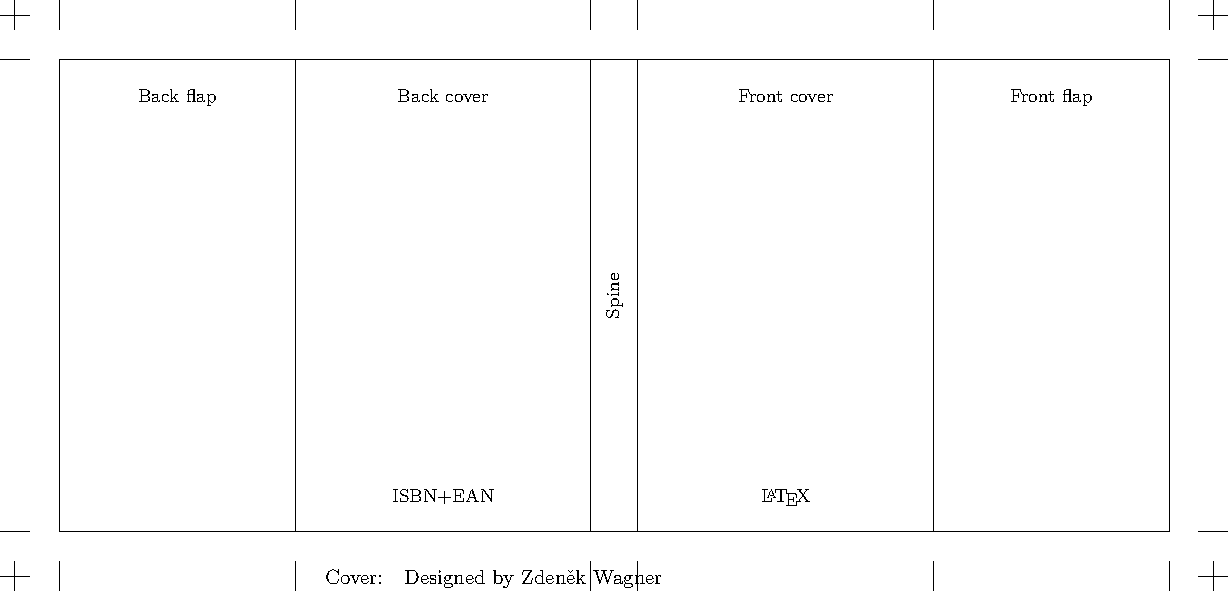
\includegraphics{coversample}}

\caption{Sample of a book cover with flaps}\label{cover}
\end{sidewaysfigure}

Remember that these macros contain only the dimensions that were specified in the \cmd{usepackage}
command, not those that were calculated by the algorithm described in section~\ref{calc.pg.layout}.
If a shortcut option was used, all real dimensions are defined, \ie. the \opt{margins} option fills
all four margin options, \opt{topmargin}, \opt{leftmargin}, \opt{rightmargin}, \opt{botmargin}, and
the \opt{trim} option fills both \opt{xtrim} and \opt{ytrim}. You can take advantage of it to make
your document more general. You can \eg. define the book cover in two variants, with or without
flaps, using this trick:

\vb
\begin{verbatim}
\ifcat$\CropFlap$
  % no flaps
\else
  \vbox to \textheight{\hsize\CropFlap
    Flap text
  }\hss
\fi
\end{verbatim}

\vb

\cmg{thePageNumber}
Macro \cmd{thePageNumber} is used to print the page number together with the crop mark text. We have
already shownd that it may be suppressed by the \opt{nopagenumbers} option. Another possibility is
to redefine it. We can \eg. define the book title with the \opt{croptitle} option and use the
text ``Cover'' instead of the page number when typesetting the cover. Usage of this macro is also
demonstrated in Figure~\ref{cover}.

\subsection{Driver switching macros}\label{driver.switching}
These macros provides conditional branching according to the currently selected driver no matter
whether it is chosen automatically or by specifying the \opt{driver} option described in
section~\ref{driver.selection}. The macros do not change page layout, they are therefore available
even if the \opt{onlycropmarks} option was given.

\cmg{ifcaseZWdriver}
Macro \cmd{ifcaseZWdriver} expands to an open \cmd{ifcase} primitive. You can thus branch the code
according to the driver. The numeric values are 0 for \texttt{unknown}, 1 for \texttt{pdftex}, 2
for \texttt{xetex}, 3 for \texttt{dvips}. The branching may look as follows:

\vb
\begin{verbatim}
\ifcaseZWdriver
  Code for unknown
\or
  Code for pdftex
\or
  Code for xetex
\or
  Code for dvips
\else
  Error, it may not happen!
\fi
\end{verbatim}

\vb
Since \cmd{ifcaseZWdriver} is a macro, it cannot be used inside another conditional statement. If
it falls to the \false\ branch, it will not be expanded and \TeX\ will complain that it sees
misplaced \cmd{else} etc. You would have to enter all corresponding contidional as \cmd{csname}
constructions or define the condition in a separate macro that will be invoked from the condition.

\textbf{Important note:} It is not guaranteed that the numerical assignment will be kept unchanched
in future versions.

\cmg{ZWifdriver}
The \cmd{ZWifdriver} allows conditional execution of a code for a specified driver. It requires two
parameters. The first parameter is the driver name, the second parameter is the code to be
executed. The macro recognizes all driver names and aliases as given in
section~\ref{driver.selection}. It can be used \eg. in cases when you have to perform some action
for a specific driver only. Suppose that you do not want to set the page bounding boxes
(see~\ref{Bboxes}) if \texttt{dvips} is used but want to set them if the same document is
processed by any other driver. You can thus put the following command to the preamble of the
document:

\vb \noindent
\verb.\ZWifdriver{dvips}{\noBboxes}.

\vb
\textbf{Note:} This macro does not depend on the numerical assignment given above. It will
therefore work the same way in the future versions.

\section{Customizing crop styles}
This section is intended for real \TeX perts. The package tries to provide a lot of options that
enable to customize the default crop style. Try to live with them because here you are touching the
very guts of the package. If you squeeze them badly, your document will suffer from strange
problems the source of which will be difficult to trace. However, if you like tough challenges and
your stomach is strong enough, then read on, but remember, you have been warned.

You ask for a different crop style by the \opt{cropstyle} option as described in
section~\ref{cropstyle} on page~\pageref{cropstyle}. Assume that you load the package with:

\vb
\begin{verbatim}
\usepackage[cropmarks,cropstyle=special,...]{zwpagelayout}
\end{verbatim}

\cmg{cropstyle@special}
You will then have to define macro \cmd{cropstyle@special}. The package first patches the footer in
all page styles. A zero-width, zero-height, zero-depth box is added to the beginning of the footer.
The actual point is set to the lower left corner of the paper as defined by \cmd{paperheight} and
\cmd{paperwidth}. If \opt{nobleedclip} was not used, the area outside the bleed box is erased. The
current color is set according to \opt{cropcolor} option and the font is selected. Afterwards the
\cmd{cropstyle@special} macro is called.

Some crop styles may require initialization. If it is the case of your style, you have to define
macro \cmd{cropstyle@special@setup}. This macro will be executed in the \cmd{AtBeginDocument} hook.
Execution of the macro in that hook allows you to defin the crop style in a package that may be
loaded after \pkg{zwpagelayout}.
It is not an error if the setup macro does not exist.

As already noted, the intention is to discourage users from writing their own crop styles. We will
therefore only mention that the package defines a few useful macros that can be used in the crop
style definition. If your temptation to design your own crop style is really strong, you should
better study the package internals yourself.

\section{Summary of driver specific features}
The driver specific features are described throughout the manual but it may not be clear from the
option or macro description that it is driver dependent. These features with the reference to the
section, where it is described, are written below. All these features are disabled if an
\texttt{unknown} driver is being used (section~\ref{driver.selection}).
\begin{itemize}
\item Page bounding boxes, section~\ref{Bboxes}
\item Page reflection, section~\ref{reflection}
\item Overprinting, section~\ref{overprinting}
\item Setting PDF information, section~\ref{pdfinfo}
\item PDF/X-1a compliance, section~\ref{pdfx1a}
\end{itemize}
Color support is, of course, driver dependent too. However, the \pkg{zwpagelayout} has no
pretention to deal with it. It is fully handled within the \pkg{color} package.

\section{Known bugs and unimplemented features}
This section describes features that are known not to work in all case or those that do not work with
all drivers.

\subsection{Driver repertoire}
Only a few most frequent drivers are automatically detected and supported. Their list is presented
in section~\ref{driver.selection}. If you use another driver, you should probably disable all
driver specific features.

\subsection{Shifted cropmarks when the running foot overflows}
If there is not enough space for the running foot, the cropmarks will most likely be shifted. It
usually happens if you set option \opt{footskip} to zero (which is its default value) and forget to
use \verb.\pagestyle{empty}..

\subsection{Page boxes and Adobe Distiller}
Setting page boxes causes a fatal error in Adobe Distiller (verified with versions 4 and~9). See
section~\ref{Bboxes}.

\subsection{Page reflection}
Option \opt{ReflectVertically} seems to produce slightly shifted output. If any of these options is
used in \XeTeX\ or more specifically with (x)dvipdfm(x) drivers, other \texttt{bop} or \texttt{eop}
code must not be used. See section~\ref{reflection} for details on its implementation.

\subsection{Overprinting}
Overprinting works in (x)dvipdfm(x) drivers but may be cumbersome in some situations. More details
are given in section~\ref{overprinting}.

It was also found that overprinting does not work if the PostScript file is converted to PDF by
GhostScript version~7.x. This is a bug in GhostScript, overprinting works fine if
GhostScript~8.x is used.

The effect of oveprinting was tested in Adobe Acrobat~9 Pro in MS~Windows~XP Home Service Pack~3.

\subsection{Inconsistent dates}
Values of \texttt{CreationDate} and \texttt{ModDate} (see section~\ref{pdfinfo}) supplied by the driver contain information on
the time zone. Unfortunatelly, time zone setting is not available in \TeX. If both fields come from
the same origin, they are set consistently. If one of them is set by the driver and the other by
the \pkg{zwpagelayout} package, then only the field set by he driver will contain the time zone
value. Depending on your time zone it may look as if the document were modified before it was
created.

\subsection{PDF/X conformance}
The PDF/X conformance is only partial. The details are given in section~\ref{pdfx1a} and its
subsections.

\section{Changes}
This section summarizes the changes. The version and the package date is given. It may be useful to
specify the date in the \cmd{usepackage} or \cmd{RequirePackage} command if you rely on a specific
feature not available in the old version of the package.

\subsection{Version 1.4c, 2013/01/13}
Bug fix, the PDF boxes are properly set even in the (x)dvipdfm(x) family of drivers, i.\,e.\@ in
\XeLaTeX.

\subsection{Version 1.4b, 2012/10/04}
New feature, the color name in the cropmarks can be displayed in white on a colored background, see
page~\pageref{color}.

\subsection{Version 1.4a, 2012/05/20}
Bug fix, if a user requested unexistent page style, the cropmark mechanism looped forever until all
main memory was exhausted. Now the package issues an error message and uses the ``empty'' page
style.

\subsection{Version 1.4, 2012/05/13}
Black overprint is implemented for the (x)dvipdfm(x) family of drivers. It means that it now works
in \XeLaTeX, see section~\ref{overprinting}.

\subsection{Version 1.3a, 2012/01/10}
\begin{itemize}
\item Bug fix, code rearrangement in order to prevent an error message if \opt{onlycropmarks} is
used. It leads to the following changes in the functionality:
\begin{enumerate}
\item Page size is always set in the driver specific way. It is still assumed that
\cmd{paperheight} and \cmd{paperwidth} contained correct values before the package was loaded.
\item Bounding boxes are set unless they are explicitly suppressed.
\item PDF options are honoured. It is therefore possible to request PDF/X compliance, set the PDF
title and other information. If you do not wish it, you have to suppress it explicitely by
\opt{nopdfinfo}.
\end{enumerate}
\end{itemize}

\subsection{Version 1.3, 2011/11/22}
\begin{itemize}
\item Bug fix, weird errors appeared if the \pkg{ifxetex} package was loaded previously either
directly or indirectly. Loading of both \pkg{ifpdf} and \pkg{ifxetex} packages written in a different way.
\item Bug fix, pagestyle patching redesigned (r.~409); in the previous versions the crop marks may
disapear if \cmd{pagestyle} was issued again, mainly when the \pkg{fancyhdr} package was used.
\item New feature, when defining a page style, a part of another style may now be inherited. The
following code now can be used:
\begin{verbatim}
\def\ps@mypagestyle{\ps@plain
    \def\@oddhead{\hfill My running head}\let\@evenhead\@oddhead}
\pagestyle{mypagestyle}
\end{verbatim}
\item Bug fix: \cmd{globaldefs} is set to zero for printing crop marks. If it were nonzero,
crop marks will not work and will spoil the document. \LaTeX\ users probably do not know this
primitive but who knows\,\ldots
\item Bug fix: without the \opt{twoside} class option and with asymetric margins the crop marks were
printed on wrong positions on the even pages.
\item New feature: crop marks style for leaflets added (section~\ref{cropstyle.leaflet}).
\end{itemize}

\subsection{Version 1.2, 2011/09/04}
\begin{itemize}
\item Bug fix, \cmd{fi} was missing in the definition of \cmd{ZWifdriver}.
\end{itemize}

\subsection{Version 1.1, 2010/12/21}
Two bugs were fixed and a few new features were introduced. Documentation is modified and extended as
well.
\begin{itemize}
\item Bug fix, if \cmd{pagestyle} or \cmd{thispagestyle} was issued within a group while crop marks
were active, the package often failed into an endless loop which resulted in exhausting the memory.
\item Bug fix, the code for page reflection for \texttt{dvips} did not preserve properly the old
\texttt{bop-hook}.
\item New feature, the driver can be explicitly selected (section~\ref{driver.selection}) and the
code can be branched according to the driver (section~\ref{driver.switching}).
\item New feature, page reflection implemented for (x)dvipdfm(x) drivers, \ie. for \XeTeX\
(section~\ref{reflection}).
\item New feature, CMYK and RGB colors explicitly defined (section~\ref{color}).
\item New feature, colors may be redefined to use the CMYK model (section~\ref{color}).
\item New feature, overprinting implemented for \texttt{pdftex} and \texttt{dvips}
(section~\ref{overprinting}).
\item New feature, PDF information can be set without the need of loading the \pkg{hyperref}
package (section~\ref{pdfinfo}).
\item New feature, partial PDF/X-1a compliance (section~\ref{pdfx1a}).
\end{itemize}

\subsection{Version 1.0a, 2008/12/26}
The sample files distributed with the package no longer require enc\TeX\ and private macro
packages.

\section{License}
The package can be used and distributed according to the \LaTeX\ Project Public License version~1.3 or later the
text of which can be found at the \texttt{License.txt} file in the \texttt{doc} directory or at
\url{http://www.latex-project.org/lppl.txt}

\section{Trade marks}
This document makes use of trade marks owned by Adobe Systems Incorporated and Microsoft
Corporation when refering to their products.

\end{document}
